\documentclass{article}
\usepackage[utf8]{inputenc}
\usepackage{graphicx}
\usepackage[fleqn, leqno]{mathtools} 
\usepackage{textcomp}
\usepackage{titling}
\usepackage{subfig}
\usepackage[parfill]{parskip}
\usepackage{xcolor}
\definecolor{LightGray}{gray}{0.9}
\usepackage{titlesec}
\setcounter{secnumdepth}{4}
\usepackage[a4paper,left=1cm,right=1cm,top=1cm,bottom=1.5cm,]{geometry}
\usepackage{eqparbox}
\usepackage{enumitem}
\usepackage{relsize}
\usepackage{dsfont}

\newcommand*{\vertbar}{\rule[-1ex]{0.5pt}{2.5ex}}
\newcommand*{\horzbar}{\rule[.5ex]{2.5ex}{0.5pt}}

\makeatletter
\newcommand{\leqnomode}{\tagsleft@true\let\veqno\@@leqno}
\newcommand{\reqnomode}{\tagsleft@false\let\veqno\@@eqno}
\makeatother

\counterwithin*{equation}{section}
\counterwithin*{equation}{subsection}
\counterwithin*{equation}{subsubsection}

\title{\vspace{-2cm} CS231N Assignment 1 - Probability Recap, Logistic Regression \& Softmax}
\date{\vspace{-5ex}}

\begin{document}
\maketitle

\section{Probability Recap}
\subsection{Probability Space}
Provides a formal model of a random process or "experiment"

Probability space consists of three elements $\dots$
\begin{itemize}
    \item \textit{Sample space} $\Omega$, which is the set of all possible outcomes
    \item \textit{Event space} $\mathcal{F}$, representing a set of events
        \begin{itemize}
            \item An event is a set of outcomes in the sample space
        \end{itemize}
    \item \textit{Probability function} $P$, assigns to each event in the event space a probability
\end{itemize}\vspace{0.5cm}

Take a \textbf{single} throw of a six-sided die as an example $\dots$

\begin{minipage}[c]{0.5\textwidth}
    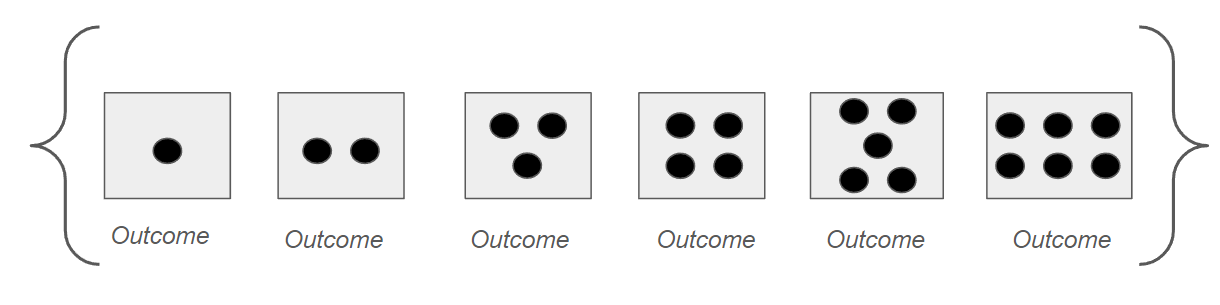
\includegraphics[width=8cm, scale=1]{images/sampleSpace.PNG}
    \captionsetup{justification=centering}
    \captionof{figure}{Sample space $\Omega$\\
                    All possible outcomes of throwing a six-sided dice \textbf{once}}
\end{minipage}%
\begin{minipage}[c]{0.5\textwidth}
    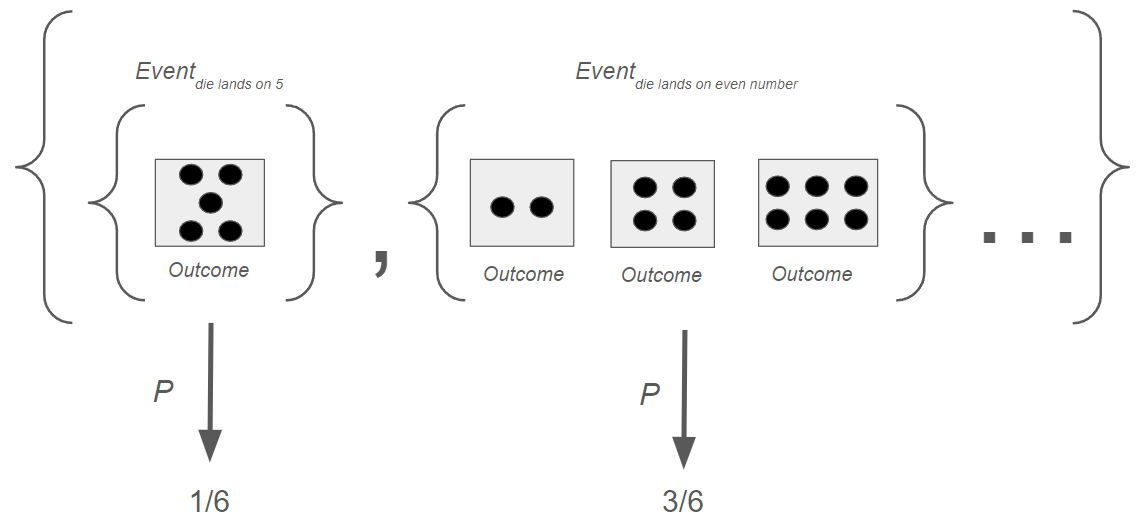
\includegraphics[width=10cm, scale=1]{images/eventSpace.PNG}
    \captionsetup{justification=centering}
    \captionof{figure}{Event space $\mathcal{F}$ could be the set of all subsets\\
                        $P$ maps each event as $\frac{\text{numOutcomes}}{6}$}
\end{minipage}%

\subsection{Random Variables}
\textit{Random variable} $\boldsymbol{X}$ is a \textbf{function} $\boldsymbol{X}:\Omega \rightarrow \mathds{R}$, from the sample space $\Omega$ to real numbers $\mathds{R}$.
Intuitively, this allows us to calculate probabilities of 'abstract' events that are happening in our sample space $\Omega$

\begin{figure}[htp]
    \centering
    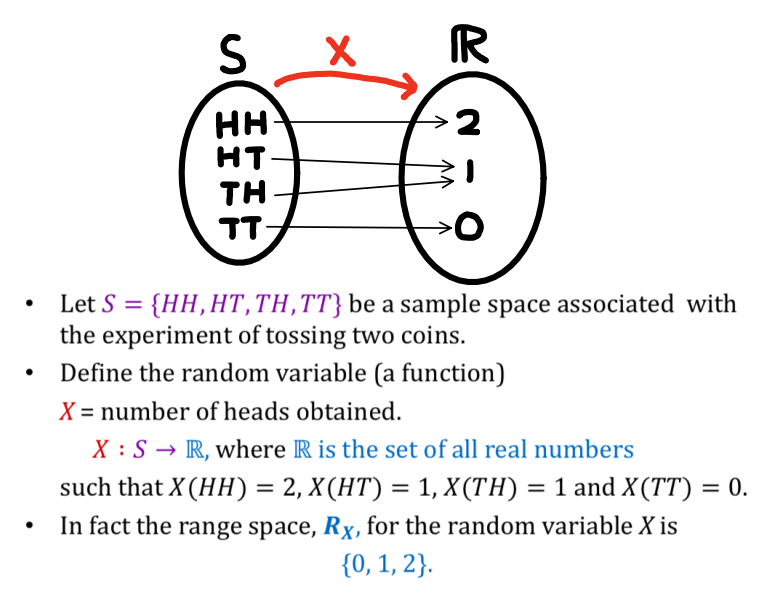
\includegraphics[width=9cm, scale=1]{images/1D_RV.PNG}
    \captionsetup{justification=centering}
    \caption{1D RV}
\end{figure}

\subsubsection{Probability distribution of an RV is not the underlying probability function}
We often specify the \textit{probability distribution} (think PMF, PDF) of a random variable directly without explicit mention of the underlying probability function defining the random variable.

In these cases, you can think of the probability function as being the probability distribution of the random variable, 
and the function defining the random variable to be the identity function.

\subsubsection{RV is not it's probability distribution}
The probability distribution of an RV is determined by $\dots$
\begin{itemize}
    \item \textbf{Underlying} probability function $P$, which represents all assumptions about our random phenomenon
    \item Random Variable $\boldsymbol{X}$ itself, ie. the function which maps sample space outcomes to real numbers in $\mathds{R}$
\end{itemize}\vspace{0.25cm}

Changing either the underlying probability function or the RV itself, will change the probability distribution of the RV.

To illustrate this point, consider the sample space $\Omega$ of two rolls of a four-sided die under the following scenarios $\dots$
\begin{enumerate}
    \item Die is fair and $\boldsymbol{X}$ is the sum of the two rolls
        \begin{itemize}
            \item $\boldsymbol{X}$ takes on value 2 with probability $\frac{1}{16}$
        \end{itemize}
    \item Die is fair and $\boldsymbol{X}$ is the larger of the two rolls
        \begin{itemize}
            \item $\boldsymbol{X}$ takes on value 2 with probability $\frac{3}{16}$
        \end{itemize}
    \item Die is weighted to land on 1 with probability 0.1, 4 with probability 0.4 and $\boldsymbol{X}$ is the sum of the two rolls
        \begin{itemize}
            \item $\boldsymbol{X}$ takes on value 2 with probability $0.01$
        \end{itemize}
\end{enumerate}

\begin{itemize}
    \item In scenario 1 and 2, the underlying probability function is the same, but the RV is different
    \item In scenario 1 and 3, the underlying probability function is different, but the RV is the same
\end{itemize}

\subsection{Expectation}

\subsubsection{Expectation of a random variable}
\begin{itemize}
    \item \textit{Probability mass function (PMF)}
        \begin{itemize}
            \item Suppose that the underlying probability function $P$ is discrete
            \item For any event $E$ containing outcomes $s$ of the sample space $\Omega$, we have that $P(E) = \sum\limits_{s \in E}p(s)$, where $p$ is the \text{PMF}
            \item Similarly, we can define $\boldsymbol{X}$ to have a PMF $p_{X}$
                \begin{itemize}
                    \item $\begin{aligned}[t]
                                p_{X}(r) &= P(X = r) \text{; Probability that $\boldsymbol{X}$ takes on some value $r \in \mathds{R}$}\\
                                         & = P({s_{i} \in \Omega} : \boldsymbol{X}(s_{i}) = r) \text{; Think of it as an event}\\
                                         & = \sum\limits_{s_{i} \in \Omega \text{ st. } \boldsymbol{X}(s_{i}) = r}p(s_{i}) \text{; Sum of all probabilities of all sample points in $\Omega$ that are assigned the value of $r$}
                            \end{aligned}$
                \end{itemize}
        \end{itemize}
    \item Expectation of a random variable $\boldsymbol{X}$
        \begin{itemize}
            \item $\begin{aligned}[t]
                        \mathds{E}[\boldsymbol{X}] &= \sum\limits_{s \in \Omega}\boldsymbol{X}(S)P\bigl(\{s\}\bigr) = \sum\limits_{s \in \Omega}\boldsymbol{X}(S)p(s)\\
                                                   &= \sum\limits_{r}rP(\boldsymbol{X}=r) = \sum\limits_{r}rp_{X}(r)
                    \end{aligned}$
        \end{itemize}
\end{itemize}

\subsubsection{Expectation of a function of a random variable}
\begin{itemize}
    \item What does $\mathlarger{\mathlarger{\mathds{E}}_{\boldsymbol{X} \sim p}[f(\boldsymbol{X})]}$ mean?
        \begin{itemize}
            \item Note that $\boldsymbol{X}$ is a random variable, \textbf{not} the \textit{realization} of the random variable
            \item $\boldsymbol{X} \sim p$ means that RV $\boldsymbol{X}$ is distributed according to some PMF/PDF $p(\boldsymbol{X})$. Note that $p$ is \textbf{not} referring to the underlying probability function $P$
            \item f$(\boldsymbol{X})$ is a \textbf{function} of the random variable $\boldsymbol{X}$
            \item Therefore, we want the expected value of $f(\boldsymbol{X})$ if $\boldsymbol{X}$ is distributed according to $p$ (ie. expectation of the \textbf{function} of an RV, closely related to expectation of an RV)
        \end{itemize}
    \item Probability distribution (PMF,PDF) is not a random variable
        \begin{itemize}
            \item Suppose we have a RV $\boldsymbol{X}$ with associated PMF $p_{X}$
            \item $p_{X}(r)$ is not an RV. It's simply a function assigning RV values to probabilities (there is nothing random happening)
            \item However, $p_{X}(\boldsymbol{X})$ is another RV (since it is a function of the RV $\boldsymbol{X}$)
        \end{itemize}
\end{itemize}

\newpage
\section{Recap on Logistic Regression}
Logistic \textit{regression} is used to solve \textit{classification} problems

\subsection{Entropy, Cross Entropy, KL Divergence}
\begin{itemize}
    \item \textit{Entropy of a \textbf{random variable}} is the average level of "information" inherent to a variable's possible outcomes
        \begin{itemize}
            \item Suppose we have discrete RV $\boldsymbol{X}$, which takes in values (outcomes) $x$ in the set $\Omega$ and is distributed according to $p_{X}: \Omega \rightarrow[0,1]$ (ie. $p_{X}$ is the PMF)
            \item  $\begin{aligned}[t]
                        \text{Define entropy of random variable as } H(\boldsymbol{X}) & := -\sum\limits_{x \in \mathds{R}}p_{X}(x)\ log\ p_{X}(x) \hspace{1cm} \text{; Expectation of negative log probability}\\
                                                                                       & := \mathds{E}_{\boldsymbol{X} \sim p_{X}}[f(\boldsymbol{X})] \hspace{2.3cm} \text{; Formulation from Expectation POV}\\
                                                                                       & := \mathds{E}_{\boldsymbol{X} \sim p_{X}}\bigl[log(p_{X}(\boldsymbol{X}))\bigr] \hspace{1.25cm} \text{; Define } f = -log(p_{X})\\
                                                                                       & := \mathds{E}_{\boldsymbol{X} \sim p_{X}}\bigl[\boldsymbol{Y}\bigr] \hspace{2.75cm} ; \ \boldsymbol{Y} = log(p_{X}(\boldsymbol{X})), \text{ our new RV}\\
                                                                                       & \ = \sum\limits_{t}\Bigl\{t*p_{Y}(t) \Bigr\}  \hspace{2.2cm} ;\ t \in image\bigl(\boldsymbol{Y}\bigr) \\
                                                                                       & \ = t_{1}p_{Y}(t_{1}) + t_{2}p_{Y}(t_{2}) + \dots \\
                                                                                       & \ = -log(p_{X}(r_{1}))*p_{Y}(t_{1}) - log(p_{X}(r_{2}))*p_{Y}(t_{2}) - \dots \\
                                                                                       & \ = -log(p_{X}(r_{1}))*p_{X}(r_{1}) - log(p_{X}(r_{2}))*p_{X}(r_{2}) - \dots \\
                                                                                       & \ = -\sum\limits_{r_{i}} log(p_{X}(r_{i}))*p_{X}(r_{i}) \hspace{0.5cm} ; \ r_{i} \in \boldsymbol{X(s_{i})}, s_{i} \in \Omega \ st. \ log(p_{X}(r_{i})) = t_{i}
                    \end{aligned}$
        \end{itemize}
    \item \textit{KL Divergence} is a measure of difference between probability distributions $P$ and $Q$. Let's not involve random variables in this discussion
        \begin{itemize}
            \item Suppose we have discrete \textbf{probability distributions} $P$ and $Q$ defined on the same sample space $\Omega$
            \item $\begin{aligned}[t]
                    D_{KL}(P || Q) & := \sum\limits_{x \in \Omega}P(x)\ log\ (\frac{P(x)}{Q(x)})\\
                                   & = -\sum\limits_{x \in \Omega}P(x)\ log\ (\frac{Q(x)}{P(x)})
                    \end{aligned}$

        \end{itemize}
    \item \textit{Cross Entropy} is another measure of difference between probability distributions $P$ and $Q$.
        \begin{itemize}
            \item A single RV cannot have multiple probability distributions (have reference material on this)
            \item Suppose we have discrete \textbf{probability distributions} $P$ and $Q$ defined on the same sample space $\Omega$
            \item \mbox{Cross Entropy is defined for two different RVs; $\boldsymbol{X}$ with probability distribution $P$, $\boldsymbol{Y}$ with probability distribution $Q$}
                \begin{itemize}
                    \item $\boldsymbol{X}$ and $\boldsymbol{Y}$ have the same image, but they create different distributions on this image (hence they are different functions).
                            $P(\boldsymbol{X}=x), Q(\boldsymbol{Y}=x)$, where $x \in \mathds{R}$
                    \item More research needs to be done on this point
                \end{itemize}
            \item $\begin{aligned}[t]
                        H(P,Q) & := -\sum\limits_{x \in \Omega}P(x)log(Q(x))
                    \end{aligned}$
        \end{itemize}
\end{itemize}

\subsubsection{Relationship between KL Divergence and Cross Entropy}
TBD\\
Have reference material on entropy of RV vs entropy of a distribution, more research needs to be done on this

\subsubsection{Derivation of Binary Cross Entropy from Cross Entropy}
TBD\\
CS3244 derives BCE from a probabilistic perspective. Let's derive BCE from Cross Entropy loss directly.

\newpage
\section{Softmax Classifier}
To be more precise, using \textit{Softmax Activation function} \textbf{minimizes} the \textit{Cross-Entropy Loss}

\begin{figure}[htp]
    \centering
    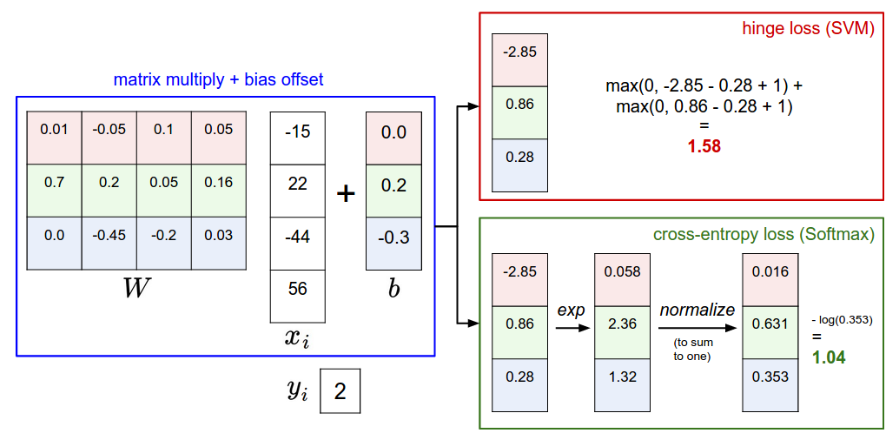
\includegraphics[width=9cm, scale=1]{images/hinge_to_cross.PNG}
    \captionsetup{justification=centering}
    \caption{SVM (\textbf{minimizing} hinge loss) vs Softmax (\textbf{minimizing} cross-entropy loss)\\
                Note that both are utilized to solve \textbf{multiclass} classification}
\end{figure}

 See CS3244 notes for more on how Softmax is minimizing cross entropy

\subsection{Numerical Stability of Softmax function}

\begin{itemize}
    \item We know that the softmax function for some datapoint $x$ is $\frac{exp(W_{(j)}^{T}x)}{\sum\limits_{i}exp(w_{(i)}^{T})x}, \ \forall j \in \{1,2, \dots, k\}$
    \item Recognize that the exponential terms may get very large, leading to numerical instability
    \item One way to rectify is this $\dots$
        \begin{itemize}
            \item[] $\begin{aligned}[t]
                        \frac{exp(W_{(j)}^{T}x)}{\sum\limits_{i}exp(w_{(i)}^{T})x} &= \frac{C * exp(W_{(j)}^{T}x)}{\sum\limits_{i}\bigl\{ C * exp(W_{(i)}^{T})x \bigr\}}\\
                                                                                   &= \frac{exp(W_{(j)}^{T}x + log (C))}{\sum\limits_{i}exp(W_{(i)}^{T}x + log(C))} \text{ ; Set $log(C) = -max(W_{(i)}^{T}x)$ (ie. Class $i$ that has largest $W_{(i)}^{T}x$ score)}
                    \end{aligned}$
        \end{itemize}
\end{itemize}

\subsection{Gradient of Softmax function}
\subsubsection{Prerequisites}
    \begin{itemize}
        \item We have training data $D = \{x_{i}, t_{i}\}_{1}^{C}$
            \begin{itemize}
                \item $C$ = number of classes
                \item $t_{i}$ = label of datapoint $x_{i}$
            \end{itemize}
        \item \textbf{Per-element} softmax function for some datapoint $x$ is $s_{i} = p(t=i\ | \ x) = 
                    \frac{exp(W_{(i)}^{T}x)}{\sum\limits_{n=1}^{C}exp(W_{(n)}^{T}x)} =
                    \frac{exp(z_{i})}{\sum\limits_{n=1}^{C}exp(z_{n})}
                    $ for $i \in \{1,2,...,C\}$ 
        \item Hence, given $W^{T} = \begin{bmatrix}
                                        \horzbar & w_{1} & \horzbar \\
                                        \horzbar & w_{2} & \horzbar \\
                                        & \vdots &\\
                                        \horzbar & w_{C} & \horzbar
                                    \end{bmatrix} \in \mathds{R}^{C x D}$ ; (D = dimension of data)
            \begin{itemize}
                \item $softmax\left(
                                \begin{bmatrix}
                                        W_{1}^{T}x\\
                                        W_{2}^{T}x\\
                                        \vdots \\
                                        W_{C}^{T}x
                                \end{bmatrix}
                              \right) = 
                        softmax\left(
                                W^{T}x
                              \right) = 
                        \begin{bmatrix}
                                P(t=1|x)\\
                                P(t=2|x)\\
                                \vdots \\
                                P(t=C|x)\\
                        \end{bmatrix}$; $softmax$: $\mathds{R}^N \rightarrow \mathds{R}^{N}$
            \end{itemize}
                \item  $\begin{aligned}[t]
                            \text{Recognize that derivative of Softmax is it's Jacobian matrix, } 
                                    J_{softmax} = 
                                    \begin{bmatrix}
                                        \frac{\partial s_{1}}{\partial z_{1}} & \frac{\partial s_{1}}{\partial z_{2}} & \dots & \frac{\partial s_{1}}{\partial z_{C}}\\
                                        \frac{\partial s_{2}}{\partial z_{1}} & \frac{\partial s_{2}}{\partial z_{2}} & \dots & \frac{\partial s_{2}}{\partial z_{C}}\\
                                        \vdots & \vdots & \ddots & \vdots\\
                                        \frac{\partial s_{C}}{\partial z_{1}} & \frac{\partial s_{C}}{\partial z_{2}} & \dots & \frac{\partial s_{C}}{\partial z_{C}}\\
                                    \end{bmatrix}
                        \end{aligned}$
    \end{itemize}

\subsubsection{Gradient Computation}
Let's consider what is $\frac{\partial s_{i}}{\partial z_{j}} = \frac{\partial }{\partial z_{j}}\frac{exp(z_{i})}{\sum\limits_{n=1}^{C}exp(z_{n})}$\\

\leqnomode
\begin{subequations}
\renewcommand{\theequation}{\theparentequation.\arabic{equation}}
    \begin{equation}
        \text{Let's consider the \textit{logarithmic derivative} (avoids the derivative quotient rule later on)}
    \end{equation}
    \begin{equation}
        \frac{\partial}{\partial z_{j}}log(s_{i}) = \frac{1}{s_{i}}\frac{\partial s_{i}}{\partial z_{j}}
    \end{equation}
    \begin{equation}
        \text{Rearranging, } \frac{\partial s_{i}}{\partial z_{j}} = s_{i} \cdot \frac{\partial}{\partial z_{j}}log(s_{i}). \text{ Observe that the LHS is the original derivative we are interested in}
    \end{equation}
\end{subequations}

\begin{subequations}
\renewcommand{\theequation}{\theparentequation.\arabic{equation}}
    \begin{equation}
        \begin{aligned}[t]
            log(s_{i}) &= log\left( \frac{exp(z_{i})}{\sum\limits_{n=1}^{C}exp(z_{n})} \right)\\
                       &= log\Bigl(exp(z_{i})\Bigr) - log \Bigl( \sum\limits_{n=1}^{C}exp(z_{n}) \Bigr)\\
                       &= z_{i} - log \Bigl( \sum\limits_{n=1}^{C}exp(z_{n}) \Bigr)
        \end{aligned}
    \end{equation}
    \begin{equation}
        \begin{aligned}[t]
            \text{Hence, } \frac{\partial}{\partial z_{j}}log(s_{i}) &= \frac{\partial}{\partial z_{j}} \Bigl\{ z_{i} - log \Bigl( \sum\limits_{n=1}^{C}exp(z_{n}) \Bigr) \Bigr\}\\
                                                                     &= \frac{\partial z_{i}}{\partial z_{j}} - \frac{\partial}{\partial z_{j}} \Bigl\{log \Bigl( \sum\limits_{n=1}^{C}exp(z_{n}) \Bigr) \Bigr\}
        \end{aligned}
    \end{equation}
    \begin{equation}
        \text{Notice that } \frac{\partial z_{i}}{\partial z_{j}} = 
            \begin{cases}
                1 \text{ if i=j}\\
                0 \text{ if i $\neq $ j}
            \end{cases}
    \end{equation}
    \begin{equation}
        \begin{aligned}[t]
            \text{Thus, } \frac{\partial}{\partial z_{j}}log(s_{i}) &= \mathds{1}_{i=j} - \frac{\partial}{\partial z_{j}} \Bigl\{log \Bigl( \sum\limits_{n=1}^{C}exp(z_{n}) \Bigr) \Bigr\}\\
                                                                    &= \mathds{1}_{i=j} - \frac{1}{\sum\limits_{n=1}^{C}exp(z_{n})} \cdot \left( \frac{\partial}{\partial z_{j}}\sum\limits_{n=1}^{C}exp(z_{n}) \right)\\
                                                                    &= \mathds{1}_{i=j} - \frac{1}{\sum\limits_{n=1}^{C}exp(z_{n})} \cdot \left( \frac{\partial}{\partial z_{j}} \Bigl\{ e^{z_{1}} + e^{z_{2}} + \dots + e^{z_{C}} \Bigr\} \right)\\
                                                                    &= \mathds{1}_{i=j} - \frac{1}{\sum\limits_{n=1}^{C}exp(z_{n})} \cdot e^{z_{j}}\\
                                                                    &= \mathds{1}_{i=j} - s_{j}
        \end{aligned}
    \end{equation}
    \begin{equation}
        \begin{aligned}[t]
            &\text{Lets multiply by $s_{i}$ on both sides to make it look like (1.3)}\\
            & s_{i} \cdot \frac{\partial}{\partial z_{j}}log(s_{i}) = s_{i} \cdot \left(\mathds{1}_{i=j} - s_{j}\right)\\
            & \frac{\partial s_{i}}{\partial z_{j}} = s_{i} \cdot \left(\mathds{1}_{i=j} - s_{j}\right); \text{ This gives us the elements of $J_{softmax}$}
        \end{aligned}
    \end{equation}
\end{subequations}
\begin{equation}
    \text{$J_{softmax}$} = 
    \begin{bmatrix}
        \frac{\partial s_{1}}{\partial z_{1}} & \frac{\partial s_{1}}{\partial z_{2}} & \dots & \frac{\partial s_{1}}{\partial z_{C}}\\
        \frac{\partial s_{2}}{\partial z_{1}} & \frac{\partial s_{2}}{\partial z_{2}} & \dots & \frac{\partial s_{2}}{\partial z_{C}}\\
        \vdots & \vdots & \ddots & \vdots\\
        \frac{\partial s_{C}}{\partial z_{1}} & \frac{\partial s_{C}}{\partial z_{2}} & \dots & \frac{\partial s_{C}}{\partial z_{C}}\\
    \end{bmatrix} = 
    \begin{bmatrix}
        s_{1} \cdot (1 - s_{1}) & -(s_{1} \cdot s_{2}) & \dots & -(s_{1} \cdot s_{C})\\
        -(s_{2} \cdot s_{1}) & s_{2} \cdot (1 - s_{2}) & \dots & -(s_{2} \cdot s_{C})\\
        \vdots & \vdots & \ddots & \vdots\\
        -(s_{C} \cdot s_{1}) & -(s_{C} \cdot s_{2}) & \dots & s_{C} \cdot (1 - s_{C})
    \end{bmatrix}
\end{equation}

\newpage
\subsubsection{Backpropagation with Softmax function}

\begin{subequations}
    \renewcommand{\theequation}{\theparentequation.\arabic{equation}}
    \begin{equation}
        \text{We know that } \frac{\partial s_{i}}{\partial z_{j}} = s_{i} \cdot (\mathds{1}_{i=j} - s_{j}), \text{ where $z_{j} = W_{(j)}^{T}x$}
    \end{equation}
    \begin{equation}
        \begin{aligned}[t]
            \text{Cross-Entropy Loss for a particular datapoint $n$ is } L_{n}(\boldsymbol{y}, \boldsymbol{s}) &= -\sum\limits_{i=1}^{C}y_{i} \cdot log(s_{i}); \text{ $\boldsymbol{y}$ is one-hot encoded label}\\
                                                                                                               &= -log(s_{k}); \text{ $k$ is the label of the particular datapoint $n$}
        \end{aligned}
    \end{equation}
    \begin{equation}
        \begin{aligned}[t]
            \frac{\partial L_{n}}{\partial z_{j}} &= \frac{\partial}{\partial z_{j}} \Bigl\{ -\sum\limits_{i=1}^{C}y_{i} \cdot log(s_{i}) \Bigr\}\\
                                                  &= -\frac{\partial}{\partial z_{j}} \sum\limits_{i=1}^{C} \Bigl\{ y_{i} \cdot log(s_{i}) \Bigr\} \\
                                                  &= -\sum\limits_{i=1}^{C} \Bigl\{ y_{i} \cdot \frac{\partial}{\partial z_{j}}log(s_{i}) \Bigr\}\\
                                                  &= -\sum\limits_{i=1}^{C} \Bigl\{ y_{i} \cdot \frac{1}{s_{i}} \cdot \frac{\partial s_{i}}{\partial z_{j}} \Bigr\}\\
                                                  &= -\sum\limits_{i=1}^{C} \Bigl\{ y_{i} \cdot \frac{1}{s_{i}} \cdot s_{i} \cdot (\mathds{1}_{i=j} - s_{j}) \Bigr\}\\
                                                  &= -\sum\limits_{i=1}^{C} \Bigl\{ y_{i} \cdot (\mathds{1}_{i=j} - s_{j}) \Bigr\}\\
                                                  &= -\sum\limits_{i=1}^{C} \Bigl\{ (y_{i} \cdot \mathds{1}_{i=j}) - (y_{i} \cdot s_{j}) \Bigr\} \\
                                                  &= \sum\limits_{i=1}^{C} \Bigl\{ (y_{i} \cdot s_{j}) - (y_{i} \cdot \mathds{1}_{i=j}) \Bigr\} \\
                                                  &= \sum\limits_{i=1}^{C} \Bigl\{ (y_{i} \cdot s_{j}) - y_{j} \Bigr\} \\
                                                  &= \sum\limits_{i=1}^{C} (y_{i} \cdot s_{j}) - \sum\limits_{i=1}^{C} y_{j} \\
                                                  &= s_{j}\sum\limits_{i=1}^{C} y_{i} - y_{j}\\
                                                  &= s_{j} - y_{j} \text{ ; Since $\boldsymbol{y}$ is a one-hot encoded vector}\\
                                                  &= s_{j} - \mathds{1}_{n=j}(1) \text{ ; $y_{j}$ (class label of score $z_{j}$) is only '1' if class label of datapoint $n$ is the same}
        \end{aligned}
    \end{equation}
    \begin{equation}
        \begin{aligned}[t]
            \frac{\partial L_{n}}{\partial W_{(j)}} &= \frac{\partial L_{n}}{\partial z_{j}} \cdot \frac{\partial z_{j}}{W_{(j)}}\\
                                                    &= (s_{j} - \mathds{1}_{n=j}(1)) \cdot x
        \end{aligned}
    \end{equation}
\end{subequations}

\newpage
\subsubsection{Gradient Computation - Vectorized}
\begin{subequations}
    \renewcommand{\theequation}{\theparentequation.\arabic{equation}}
    \begin{equation}
       \text{Denote our minibatch of data as } \boldsymbol{X} = \begin{bmatrix}
                                                                    \horzbar x_{1} \horzbar\\
                                                                    \horzbar x_{2} \horzbar\\
                                                                    \dots \\
                                                                    \horzbar x_{N} \horzbar
                                                                \end{bmatrix}
        \in \mathds{R}^{NxD} \text{ ; $N$ = number of samples, $D$ = dimension of data}
    \end{equation}
    \begin{equation}
       \text{Denote our weight matrix as } \boldsymbol{W} = \begin{bmatrix}
                                                                \vertbar & \vertbar & \vertbar & \vertbar \\
                                                                w_{1}    & w_{2}    & \hdots & w_{C} \\
                                                                \vertbar & \vertbar & \vertbar & \vertbar
                                                            \end{bmatrix}
       \in \mathds{R}^{DxC} \text{ ; C = number of classes}
    \end{equation}
    \begin{equation}
        \begin{aligned}[t]
            \text{Denote our softmax function as } \boldsymbol{s} =
                \begin{bmatrix}
                   s_{1}\\
                   s_{2}\\
                   \hdots\\
                   s_{C}
                \end{bmatrix} \text{, where } s_{i} = p(t=i\ | \ x) = \frac{exp(W_{(i)}^{T}x)}{\sum\limits_{n=1}^{C}exp(W_{(n)}^{T}x)} = \frac{exp(z_{i})}{\sum\limits_{n=1}^{C}exp(z_{n})}
        \end{aligned}
    \end{equation}
    \begin{equation}
        \begin{aligned}[t]
            \text{For a single datapoint $x_{n} \in \mathds{R}^{1xD}$ , } \frac{\partial L_{n}}{\partial \boldsymbol{W}} 
            &= 
            \begin{bmatrix}
                \vertbar & \vertbar & \vertbar & \vertbar \\
                \frac{\partial L_{n}}{\partial W_{(1)}} &  \frac{\partial L_{n}}{\partial W_{(2)}} & \dots & \frac{\partial L_{n}}{\partial W_{(C)}} \\
                \vertbar & \vertbar & \vertbar & \vertbar
            \end{bmatrix} \in \mathds{R}^{DxC}\\
            &= 
            \begin{bmatrix}
                \vertbar & \vertbar & \vertbar & \vertbar \\
                (s_{1} - \mathds{1}_{i=1}) \cdot x_{n} & (s_{2} - \mathds{1}_{i=2}) \cdot x_{n} & \dots & (s_{C} - \mathds{1}_{i=C}) \cdot x_{n}\\
                \vertbar & \vertbar & \vertbar & \vertbar
            \end{bmatrix}\\
            &= 
            \begin{bmatrix}
                (s_{1} - \mathds{1}_{i=1}) \cdot x_{n_{1}} & (s_{2} - \mathds{1}_{i=2}) \cdot x_{n_{1}} & \dots & (s_{C} - \mathds{1}_{i=C}) \cdot x_{n_{1}}\\
                (s_{1} - \mathds{1}_{i=1}) \cdot x_{n_{2}} & (s_{2} - \mathds{1}_{i=2}) \cdot x_{n_{2}} & \dots & (s_{C} - \mathds{1}_{i=C}) \cdot x_{n_{2}}\\
                \vdots & \vdots & \ddots & \vdots\\
                (s_{1} - \mathds{1}_{i=1}) \cdot x_{n_{D}} & (s_{2} - \mathds{1}_{i=2}) \cdot x_{n_{D}} & \dots & (s_{C} - \mathds{1}_{i=C}) \cdot x_{n_{D}}\\
            \end{bmatrix}\\
            &=
            \begin{bmatrix}
                x_{n_{1}}\\
                x_{n_{2}}\\
                \dots\\
                x_{n_{D}}
            \end{bmatrix} \cdot
            \begin{bmatrix}
                (s_{1} - \mathds{1}_{i=1}) \ \ \ (s_{2} - \mathds{1}_{i=2}) \ \ \ \dots \ \ \ (s_{C} - \mathds{1}_{i=C})
            \end{bmatrix}\\
            &=
            x_{n}^{T} \cdot 
            \begin{bmatrix}
                (s_{1} - \mathds{1}_{i=1}) \ \ \ (s_{2} - \mathds{1}_{i=2}) \ \ \ \dots \ \ \ (s_{C} - \mathds{1}_{i=C})
            \end{bmatrix}\\
        \end{aligned}
    \end{equation}
    \begin{equation}
        \text{For all datapoints $\boldsymbol{X} \in \mathds{R}^{NxD}$ , we have } \frac{\partial L}{\partial \boldsymbol{W}} \in \mathds{R}^{DxC} \text{; Shape makes sense (think about it)}
    \end{equation}
    \begin{equation}
        \begin{aligned}[t]
            \frac{\partial L}{\partial \boldsymbol{W}} &= \frac{1}{N} \sum\limits_{i}\frac{\partial L_{i}}{\partial \boldsymbol{W}} \\&=
            \begin{bmatrix}
                x_{1_{1}}\\
                x_{1_{2}}\\
                \dots\\
                x_{1_{D}}
            \end{bmatrix} \cdot
            \begin{bmatrix}
                (s_{1} - \mathds{1}_{i=1})_{1} \ (s_{2} - \mathds{1}_{i=2})_{2} \ \dots \ (s_{C} - \mathds{1}_{i=C})_{N}
            \end{bmatrix} +
            \begin{bmatrix}
                x_{2_{1}}\\
                x_{2_{2}}\\
                \dots\\
                x_{2_{D}}
            \end{bmatrix} \cdot
            \begin{bmatrix}
                (s_{1} - \mathds{1}_{i=1})_{2} \ (s_{2} - \mathds{1}_{i=2})_{2} \ \dots \ (s_{C} - \mathds{1}_{i=C})_{2}
            \end{bmatrix} +
            \dots
            \\&=
            \begin{bmatrix}
                x_{1_{1}}(s_{1} - \mathds{1}_{i=1})_{1} + x_{2_{1}}(s_{1} - \mathds{1}_{i=1})_{2} + \dots + x_{N_{1}}(s_{1} - \mathds{1}_{i=1})_{N}\\
                x_{1_{2}}(s_{1} - \mathds{1}_{i=1})_{1} + x_{2_{2}}(s_{1} - \mathds{1}_{i=1})_{2} + \dots + x_{N_{2}}(s_{1} - \mathds{1}_{i=1})_{N}\\
                \dots\\
                x_{1_{D}}(s_{1} - \mathds{1}_{i=1})_{1} + x_{2_{D}}(s_{1} - \mathds{1}_{i=1})_{2} + \dots + x_{N_{D}}(s_{1} - \mathds{1}_{i=1})_{N}\\
            \end{bmatrix}\\ &=
            \begin{bmatrix}
                x_{1_{1}} & x_{2_{1}} & \dots & x_{N_{1}} \\
                x_{1_{2}} & x_{2_{2}} & \dots & x_{N_{2}} \\
                \vdots    & \vdots    & \ddots & \vdots \\
                x_{1_{D}} & x_{2_{D}} & \dots & x_{N_{D}} \\
            \end{bmatrix} \cdot
            \begin{bmatrix}
                (s_{1} - \mathds{1}_{i=1})_{1} \ \ \ & (s_{2} - \mathds{1}_{i=2})_{1} \ \ \ & \dots \ \ \ & (s_{C} - \mathds{1}_{i=C})_{1}\\
                (s_{1} - \mathds{1}_{i=1})_{2} \ \ \ & (s_{2} - \mathds{1}_{i=2})_{2} \ \ \ & \dots \ \ \ & (s_{C} - \mathds{1}_{i=C})_{2}\\
                \vdots    & \vdots    & \ddots & \vdots \\
                (s_{1} - \mathds{1}_{i=1})_{N} \ \ \ & (s_{2} - \mathds{1}_{i=2})_{N} \ \ \ & \dots \ \ \ & (s_{C} - \mathds{1}_{i=C})_{N}
            \end{bmatrix}\\ &=
            \begin{bmatrix}
                \vertbar & \vertbar & \vertbar & \vertbar \\
                x_{1}    & x_{2}    & \hdots & x_{N} \\
                \vertbar & \vertbar & \vertbar & \vertbar
            \end{bmatrix} \cdot
            \begin{bmatrix}
                \vertbar & \vertbar & \vertbar & \vertbar \\
                (s_{1}-\mathds{1}_{i=1})_{1 \dots N} & (s_{2}-\mathds{1}_{i=2})_{1 \dots N} & \hdots & (s_{C}-\mathds{1}_{i=C})_{1 \dots N} \\
                \vertbar & \vertbar & \vertbar & \vertbar
            \end{bmatrix}\\ &=
            \begin{bmatrix}
                \vertbar & \vertbar & \vertbar & \vertbar \\
                x_{1}    & x_{2}    & \hdots & x_{N} \\
                \vertbar & \vertbar & \vertbar & \vertbar
            \end{bmatrix} \cdot
            \begin{bmatrix}
                \horzbar \ &(\boldsymbol{s} - \mathds{1}_{i=1 \dots C})_{1} &\ \horzbar \\
                \horzbar \ &(\boldsymbol{s} - \mathds{1}_{i=1 \dots C})_{2} &\ \horzbar \\
                \horzbar \ & \dots\dots\dots\dots\dots & \ \horzbar \\
                \horzbar \ &(\boldsymbol{s} - \mathds{1}_{i=1 \dots C})_{N} &\ \horzbar \\
            \end{bmatrix}\\ &=
            \boldsymbol{X}^{T}\boldsymbol{Q} \text{; Where $\boldsymbol{Q}$ is defined as above}
        \end{aligned}
    \end{equation}
\end{subequations}

\end{document}